\documentclass[12pt,twocolumn]{IEEEtran}

\usepackage{ucs}
\usepackage[utf8]{inputenc}
\usepackage{xcolor}
\usepackage{fontenc}
%\usepackage[showframe]{geometry}
\usepackage{graphicx}
%\usepackage{multicol}
%\usepackage{lipsum}
%\usepackage{minted}
%\usemintedstyle{monokai}
\usepackage{float}
\usepackage[dvips]{hyperref}

%\author{Aravind}
\title{I2C Protocol}
\date{02/05/2017}
 
\begin{document}
 %With \verb!\_!:
  \maketitle
    \section{The physical I2C bus}
    SCL is the clock line. It is used to synchronize all data transfers over the I2C bus. SDA is the data line. The SCL and SDA lines are connected to all devices 
    on the I2C bus.

  \subsection{Masters and Slaves}
      The devices on the I2C bus are either masters or slaves. The master is always the device that drives the SCL clock line. The slaves are the devices that 
      respond to the master. There can be, and usually are, multiple slaves on the I2C bus.Slaves will never initiate a transfer. Both master and slave can transfer 
      data over the I2C bus, but that transfer is always controlled by the master.

  \begin{figure}[p]
    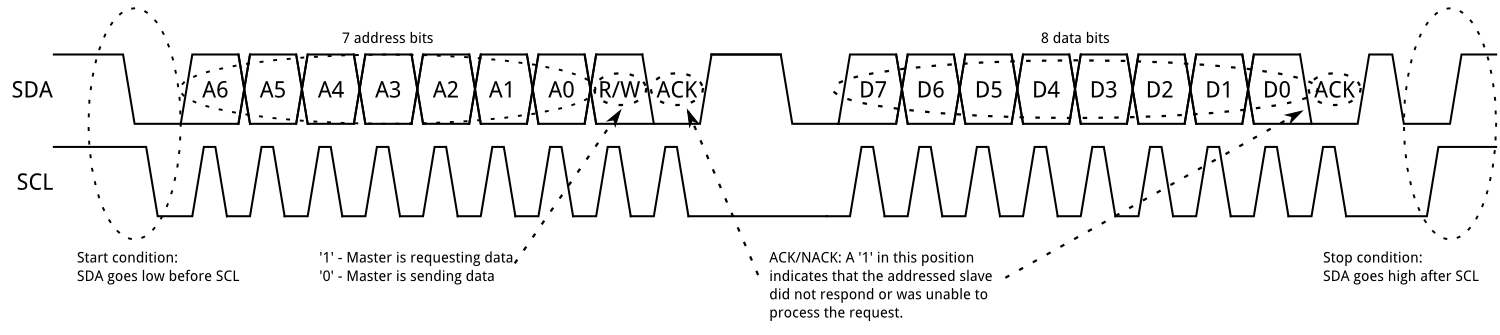
\includegraphics[width=\textwidth]{i2c_concept.png}
    \caption{The I2C protocol}
  \end{figure}


  \section{The I2C Physical Protocol}

    Data is transferred in sequences of 8 bits. The bits are placed on the SDA line starting with the MSB (Most Significant Bit). The SCL line is then) pulsed 
high, then low.For every 8 bits transferred, the slave receiving the data sends back an acknowledge bit, so there are actually 9 SCL clock pulses to transfer 
each byte of data. If the slave sends back a low ACK bit, then it has received the data and is ready to accept another byte. If a high sent, then it indicates
no further data can be accepted. 
A start sequence is one of two special sequences defined for the I2C bus, the other being the stop sequence. The start sequence and stop sequence are special 
in that these are the only places where the SDA (data line) is allowed to change while the SCL (clock line) is high. When data is being transferred, SDA must
remain stable and not change whilst SCL is high. The start and stop sequences mark the beginning and end of a transaction with the slave device.

  \begin{figure}[H]
    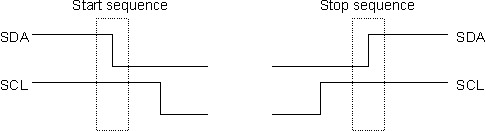
\includegraphics[width=0.5\linewidth]{start_stop_seq.jpeg}
  \end{figure}




    \subsection{I2C Device Addressing}
	Here the I2C address is made of 7 bits. When sending out the 7 bit address, we still always send 8 bits. The extra bit is used to inform the slave if the master is  writing to it or reading from it. If the R/W bit is '0' the master is writing to the slave. If the bit is '1' the master is reading from the slave. The 7 bit address is placed in the upper 7 bits of the byte and the Read/Write (R/W) bit is in the LSB (Least Significant Bit).

  \section{Theory of Operation}
    The I2C master we implemented uses the state machine depicted in Figure 1 to implement the I2C-bus protocol. Upon start-up, the component immediately
    enters the ready state(here, enters and remains in idle state till an edge trigger happens). 

    Once an edge trigger happens the start state generates the start condition on the I2C bus, and the command state communicates the address(start\_addr\_tx) 
    and rw command to the bus. 

    The slv\_ack1 state(slave\_hit\_addr) then captures and verifies the slave’s acknowledgment(ack\_one), if not acknowledged goes back to idle state. 

    Depending on the rw command, the component then proceeds to either write data to the slave (wr state) or receive data from the slave (rd state). 
    In our implementation, we have dealt with write only. If it hits read,it goes back to idle state.

    Once state\_reg hits write, it will keep receiving bits of data to write to slave till bit\_cnt reaches 7 (8 bits of data sent).

    Once bit\_cnt equals 8, depending on the acknowledgment we receive from slave\_hit\_data , the state either ends the process (ack\_two =0) or goes back 
    to idle state(ack\_two =1). 

    Once the process has finished running successfully (i.e. ack\_two =0) it goes back to idle state and waits for the edge trigger (sda). If sda is received 
    as 1, then our I2C repeats the process over again from start.

  
 % \begin{minted}[
%     frame=lines,
%     framesep=2mm,
%     bgcolor=LightGray,
%     fontsize=\footnotesize,
%     linenos
%   ]{vhdl}
% -----------------
% ----code here
% -----------------
%   \end{minted}

\end{document}


